% Template created by Karol Kozioł (www.karol-koziol.net) for ShareLaTeX
\documentclass[a4paper,9pt]{extarticle}

\usepackage[utf8]{inputenc}
\usepackage[T1]{fontenc}
\usepackage{graphicx}
\usepackage{xcolor}
\usepackage{tikz}

\usepackage{amsmath,amssymb,textcomp}
\everymath{\displaystyle}

\usepackage{times}
\renewcommand\familydefault{\sfdefault}
\usepackage{tgheros}
% \usepackage[defaultmono,scale=0.85]{droidmono}

\usepackage{multicol}
\setlength{\columnseprule}{0pt}
\setlength{\columnsep}{20.0pt}

\usepackage{xeCJK}


\usepackage{listings}
\usepackage{xcolor}

\definecolor{codegreen}{rgb}{0,0.6,0}
\definecolor{codegray}{rgb}{0.5,0.5,0.5}
\definecolor{codepurple}{rgb}{0.58,0,0.82}
\definecolor{backcolour}{rgb}{0.95,0.95,0.92}

\lstdefinestyle{mystyle}{
    backgroundcolor=\color{backcolour},   
    commentstyle=\color{codegreen},
    keywordstyle=\color{magenta},
    numberstyle=\tiny\color{codegray},
    stringstyle=\color{codepurple},
    basicstyle=\ttfamily\footnotesize,
    breakatwhitespace=false,         
    breaklines=true,                 
    captionpos=b,                    
    keepspaces=true,                 
    numbers=left,                    
    numbersep=5pt,                  
    showspaces=false,                
    showstringspaces=false,
    showtabs=false,                  
    tabsize=2
}
\lstset{style=mystyle}

% Box for definitions.
\usepackage{tcolorbox}
\newtcolorbox{mydef}[1]{colback=red!5!white,colframe=red!75!black,fonttitle=\bfseries,title=定义:#1}

\usepackage{amsmath}
\usepackage{amssymb}
\usepackage{amsthm}
\newtheorem{example}[section]{例}
\newtheorem{theorem}{定理}[section]
\newtheorem{corollary}{推论}[theorem]
\newtheorem{lemma}[theorem]{引理}
\newtheorem*{pr}{证明}

\usepackage{hyperref}
\usepackage{url}

\usepackage{geometry}
\geometry{a4paper,left=10mm,right=10mm,top=10mm,bottom=15mm}

\linespread{1.3}


% custom title
\makeatletter
\renewcommand*{\maketitle}{%
\noindent
\begin{minipage}{0.4\textwidth}

\begin{tikzpicture}
\node[rectangle,rounded corners=6pt,inner sep=10pt,fill=blue!50!black,text width= 0.95\textwidth] {\color{white}\Huge \@title};
\end{tikzpicture}
\end{minipage}
\hfill
\begin{minipage}{0.55\textwidth}
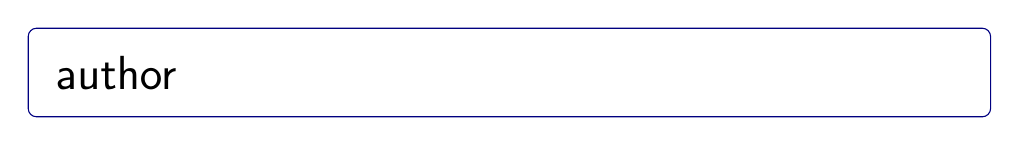
\begin{tikzpicture}
\node[rectangle,rounded corners=3pt,inner sep=10pt,draw=blue!50!black,text width= 0.95\textwidth] {\LARGE \@author};
\end{tikzpicture}
\end{minipage}
\bigskip\bigskip
}%
\makeatother

% custom section
\usepackage[explicit]{titlesec}
\newcommand*\sectionlabel{}
\titleformat{\section}
  {\gdef\sectionlabel{}
   \normalfont\sffamily\Large\bfseries\scshape}
  {\gdef\sectionlabel{\thesection\ }}{0pt}
  {
\noindent
\begin{tikzpicture}
\node[rectangle,rounded corners=3pt,inner sep=4pt,fill=blue!50!black,text width= 0.95\columnwidth] {\color{white}\sectionlabel#1};
\end{tikzpicture}
  }
\titlespacing*{\section}{0pt}{15pt}{10pt}


% custom footer
\usepackage{fancyhdr}
\makeatletter
\pagestyle{fancy}
\fancyhead{}
\fancyfoot[C]{\footnotesize \textcopyright\ \@date\ \ 本课件仅限东南大学机器学习课程使用,版权属于相关作者,严禁传播。}
\renewcommand{\headrulewidth}{0pt}
\renewcommand{\footrulewidth}{0pt}
\makeatother



\title{机器学习讲义模板}
\author{授课教师: 王贝伦  /  助教:张嘉琦,黄旭,谈笑,徐浩卿}
\date{2020}



\begin{document}

\maketitle

\begin{multicols*}{2}

\section{各级标题}
    尽量不要超过三级标题,尽量只使用 section, subsection, subsubsection。对于需要并列解释的部分,使用itemize环境。
    
    \begin{itemize}
        \item 第一条
        \item 第二条
        \item ...
    \end{itemize}
    
    
\section{基本结构}
    讲义中每一个section是一个算法/模型的解释。一个section基本结构按顺序来说是
    \begin{itemize}
        \item [(1)] 相关问题的说明:用非数学的语言说明这个方法提出的motivation是什么?可以用来解决什么样的application?
        \item [(2)] 算法/模型形式定义:详细解释这个模型的形式;说明输入、输出、损失函数形式。
        \item [(3)] 算法/模型的数学细节:从数学的角度证明算法/模型的解。这部分要详细说明这个算法/模型的数学基础以及相关数学推导(solution, theorem, error bound)。
        \item [(4)] 例子:举一个例子,用这个算法/模型对你提出的例子建模,推导针对这个例子的算法的解。
        \item [(5)]编程实现:针对你在上面提到的例子,给出编程实现的细节。代码部分需要包括数据生成,模型建立以及求解的过程。
    \end{itemize}

\section{常用环境}

\begin{mydef}{定义名称}
    对新出现的概念或者数学符号进行定义。
\end{mydef}

\begin{example}
    例子内容。
\end{example}

\begin{theorem}
    定理内容
\end{theorem}

\begin{lemma}
    引理。引理是证明一个定理需要的background。
\end{lemma}

\begin{corollary}
    推论。推论是根据一个定理推导、发散出的新的结果。
\end{corollary}

\begin{pr}
    证明。
\end{pr}


\section{数学公式}

    每个数学公式需要编号,使用equation环境,对于需要换行的数学公式,在equation内使用aligned环境。
    
    单行公式:
    \begin{equation}
        a = b + c
    \end{equation}
    
    多行公式:
    \begin{equation}
        \begin{aligned}
        & a = 1 \\
        & b = 2 \\
        & c = a + b
        \end{aligned}
    \end{equation}
    
    矩阵:
    \begin{equation}
        a = \begin{bmatrix} 
            1 & 0 \\\\
            0 & 1 
            \end{bmatrix}
    \end{equation}
\section{编程实现}
    编程代码用Python实现,并用lstlisting环境表示。
    \begin{lstlisting}[language=Python]
    import numpy as np
    
    # 加法运算
    a = 1
    b = 2
    c = a + b
    print(c)
    # Output: 3
    \end{lstlisting}
    
\section{图片与表格}
    图片用myfig环境导入。表格用mytab环境导入。图片的放在图片下方,表格的标题放在表格上方。
    每一个图片和表格都需要用标题简述内容。
	
\begin{myfig}[!htb]
  \centering
  
\includegraphics[width=\linewidth]{images.png}
  \captionof{figure}{my caption of the figure}
\end{myfig}
 
\begin{mytab}[!htb]
  \captionof{table}{Table Caption}
  \resizebox{!}{70pt}{
  \begin{tabular}{|c|c|}
    \hline
    This & is \\ \Xhline{2pt}
    a & test \\ \hline
  \end{tabular}
  }
\end{mytab}

\section{算法伪代码}
主要算法需要提供伪代码。使用algorithm环境。

\begin{algorithm}[H]
    \SetAlgoLined
    \bfseries{输入:} 样本矩阵$x \in \mathbb{R}^{n \times p}$, 样本对应的标签$y \in \mathbb{R}^n$,最大迭代次数$T$和学习率$\alpha > 0$。
     随机初始化系数向量$w$\;
     \For{$t \gets 1$ to $T$}{
       随机打乱$n$个样本的顺序\;
       \For{$i \gets 1$ to $n$}{
         $\theta \gets \theta - \alpha(y_i - x_i^\top\theta)x_i$ \; 
       }
       \If{满足停机准则}{
         break\;
       }
     }
     \bfseries{输出:} 预测系数$\theta$。
     \caption{随机梯度下降算法(SGD)}
     \label{algo:SGD}
    \end{algorithm}
 
\section*{引用}
    主要的引用需要说明,格式不需要太过正规,只要说明清楚就可以。
    \begin{itemize}
        \item [[1]] Strang, G., Strang, G., Strang, G., \& Strang, G. (1993). Introduction to linear algebra (Vol. 3). Wellesley, MA: Wellesley-Cambridge Press.
        
        \item [[2]] ABIDE: \url{http://fcon_1000.projects.nitrc.org/indi/abide/}
    \end{itemize}

\end{multicols*}
\end{document}
